%========================================================================
%
%========================================================================
\section{Les générateurs aléatoires}
\label{section:rand-gen}

   Dans un simulateur, la génération de nombres aléatoires est un
élément important. Dans {\sc ndes}, on prend ces choses-là très au
sérieux. Du coup, la gestion des nombres aléatoires est une horreur
sans nom ! J'avoue avoir moi-même du mal à comprendre. La bonne
nouvelle c'est que du coup le résultat est vraiment \ldots{}
aléatoire.

%------------------------------------------------------------------------
%
%------------------------------------------------------------------------
\subsection{Caractéristiques d'un générateur aléatoire}

   Un générateur aléatoire est caractérisé par trois composantes
fondamentales (illustrées de gauche à droite par la figure
\ref{figure:randomGenerator}.

\begin{description}
   \item[La source] permet de déterminer la qualité de l'aléa, et par
     exemple de le rendre déterministe (afin d'obtenir la même
     séquence sur plusieurs simulation).
   \item[La loi] peut être uniforme, exponentielle, \ldots
   \item[Le type des données générées] peut être réel, entier,
     discret, \ldots
\end{description}

   Attention, ces trois composantes sont éventuellement constitutées
d'un jeu de paramètres.

\begin{figure}[h]
\begin{center}
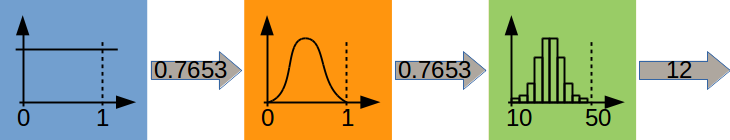
\includegraphics[width=\textwidth]{randomGenerator.png}
\caption{Structure générale d'un générateur aléatoire\label{figure:randomGenerator}}
\end{center}
\end{figure}

   Le principe général de génération d'une valeur est le suivant.

\begin{itemize}
   \item Un nombre aléatoire est fourni par la source. Ce sera un
     entier entre deux valeurs extrèmes, par exemple, en fonction de
     la nature de la source.
   \item Une transformation est appliquée afin de respecter la
     densité de probabilité de la loi.
   \item Une seconde transformation est appliquée pour obtenir une
     valeur du type voulu.
\end{itemize}

   Bref, tout est fait pour laisser sa place au hasard \ldots

   Attention, se pose ici un problème de conversion qui, très
honnètement, n'est pas encore complètement tranché !

   Les valeurs produites en sortie de l'élément qui implante la
distribution (le carré central sur la figure
\ref{figure:randomGenerator} sont comprises dans le support de la
distribution. Elles seront ensuite adaptées au type, ce qui peut
donner des choses surprenantes (et difficiles à détectées car
aléatoires !).

   Le problème essentiel vient des types intervalle. Une
transformation affine du support est réalisée, ce qui n'est
probablement pas ce que vous souhaitez. Cette transformation ne
présente d'intérêt que pour la distribution uniforme.

%------------------------------------------------------------------------
%
%------------------------------------------------------------------------
\subsection{Utilisation}

   Le schéma général d'utilisation est simple : on crée un générateur,
on l'initialise avec le type de données voulu, on lui associe une
distribution, éventuellement on peut changer la source d'aléa sur
laquelle il se fonde, puis on peut lui extirper des valeurs aléatoires
et enfin on le détruit sans un mot de remerciement.

   Observons en détail les fonctions utiles à ce programme alléchant.

%------------------------------------------------------------------------
%
%------------------------------------------------------------------------
\subsection{Création et destruction}

   Il existe au moins une fonction de création pour chaque type de
données géré (il manquerait plus que ça !). Mais il existe également
parfois des fonctions permettant de spécifier en même temps la
distribution à utiliser. Voyons ça type par type.

%.......................................................................
%
%.......................................................................
\subsubsection{Les entiers non signés}

   La fonction de création de base est 

\index{randomGenerator\_createUInt}
\begin{verbatim}
struct randomGenerator_t * randomGenerator_createUInt();
\end{verbatim}

%.......................................................................
%
%.......................................................................
\subsubsection{Les entiers non signés entre {\tt min} et {\tt max} inclus}

   Ça c'est sympa pour jouer aux dés. On les crée avec 

\begin{verbatim}
struct randomGenerator_t * randomGenerator_createUIntRange(unsigned int min,
						      unsigned int max);
\end{verbatim}

%.......................................................................
%
%.......................................................................
\subsubsection{Une liste d'entiers non signés}

   Pratique pour tirer au hasard des tailles de paquets !

\index{randomGenerator\_createUIntDiscrete}
\begin{verbatim}
struct randomGenerator_t * randomGenerator_createUIntDiscrete(int nbValues,
							      unsigned int * values);
\end{verbatim}

   Le premier paramètre donne le nombre de valeurs, et le second est
un tableau qui contient (au moins) ces valeurs. Son contenu sera
recopié, donc si tu veux le détruire/modifier ensuite, vis ta vie !

   Comme on se doute bien que dans ce genre de situations on va
vouloir associer une probabilité à chaque valeur, on peut utiliser la
version suivante :

\index{randomGenerator\_createUIntDiscreteProba}
\begin{verbatim}
struct randomGenerator_t * randomGenerator_createUIntDiscreteProba(
				int nbValues,
				unsigned int * values,
				double * proba);
\end{verbatim}

%.......................................................................
%
%.......................................................................
\subsubsection{Des réels double précision}

   On crée un tel générateur avec la fonction suivante

\index{randomGenerator\_createDouble}
\begin{verbatim}
struct randomGenerator_t * randomGenerator_createDouble();
\end{verbatim}

   On peut également en créer un fondé sur une distribution
exponentielle de paramètre {\tt lambda} :

\index{randomGenerator\_createDoubleExp}
\begin{verbatim}
struct randomGenerator_t * randomGenerator_createDoubleExp(double lambda);
\end{verbatim}

%.......................................................................
%
%.......................................................................
\subsubsection{Des réels double précision entre {\tt min} et {\tt max}}

\begin{verbatim}
\end{verbatim}

%.......................................................................
%
%.......................................................................
\subsubsection{Une liste de réels double précision}

   Pour générer des nombres aléatoires choisis dans une liste fournie
en paramètre :

\index{randomGenerator\_createDoubleDiscrete}
\begin{verbatim}
struct randomGenerator_t * randomGenerator_createDoubleDiscrete(
                                     int nbValues,
                                     double * values);
\end{verbatim}

   ou, en fournissant directement les probabilités :

\index{randomGenerator\_createDoubleDiscreteProba}
\begin{verbatim}
struct randomGenerator_t * randomGenerator_createDoubleDiscreteProba(
                                     int nbValues,
                                     double * values,
                                     double * proba);
\end{verbatim}

   Les paramètres sont analogues à la version fondée sur des entiers
non signés, bref, voir ci-dessus.

%.......................................................................
%
%.......................................................................
\subsubsection{Destruction}

   On détruit un générateur grâce à la fonction

\index{randomGenerator\_delete}
\begin{verbatim}
void randomGenerator_delete(struct randomGenerator_t * rg);
\end{verbatim}

%------------------------------------------------------------------------
%
%------------------------------------------------------------------------
\subsection{Choix de la distribution}

   Avant de pouvoir être utilisé, un générateur aléatoire doit être
caractérisé par la loi qui le gouverne. Il existe des fonctions
spécifiques à cet objectif. Certaines fonctions de création font appel
à l'une ou l'autre de ces fonctions, mais pas toute ! Attention donc à
s'assurer qu'une distribution est associée à un générateur avant de
l'utiliser.

%.......................................................................
%
%.......................................................................
\subsubsection{Distribution uniforme}

   On spécifie une loi uniforme grâce à la fonction suivante

\index{randomGenerator\_setDistributionUniform}
\begin{verbatim}
void randomGenerator_setDistributionUniform(struct randomGenerator_t * rg);
\end{verbatim}

   Attention, le type des données peut être un intervalle borné
``continu'' ou un ensemble discret, mais s'il s'agit d'un intervalle
non borné, le résultat est \ldots {} aléatoire.

   La figure \ref{figure:distuni} donne un exemple de résultat obtenu
avec une distribution uniforme réelle dans l'intervalle $[0, 1]$.

\begin{figure}[h]
\begin{center}
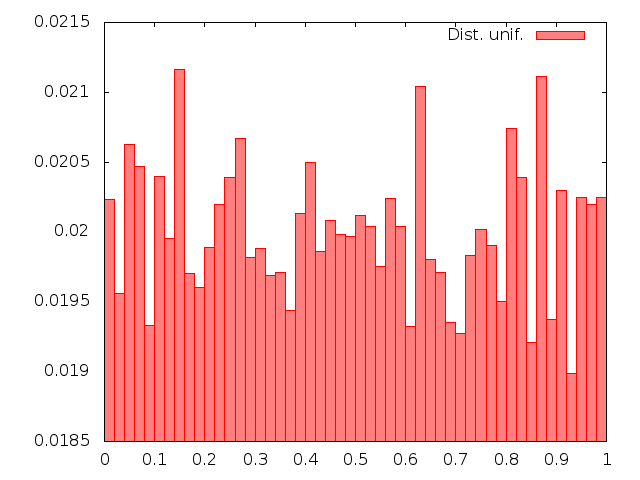
\includegraphics[width=0.5\textwidth]{DistributionUnif.png}
\caption{Une loi uniforme\label{figure:distuni}}
\end{center}
\end{figure}

%.......................................................................
%
%.......................................................................
\subsubsection{Distribution exponentielle}

   On spécifie une loi exponentielle de paramètre $\lambda$ grâce à la
fonction suivante 

\index{randomGenerator\_setDistributionExp}
\begin{verbatim}
void randomGenerator_setDistributionExp(struct randomGenerator_t * rg,
                                        double lambda);

\end{verbatim}

   La figure \ref{figure:distexp} donne un exemple de résultat obtenu
avec une distribution exponentielle de paramètre $\lambda = 10.0$

\begin{figure}[h]
\begin{center}
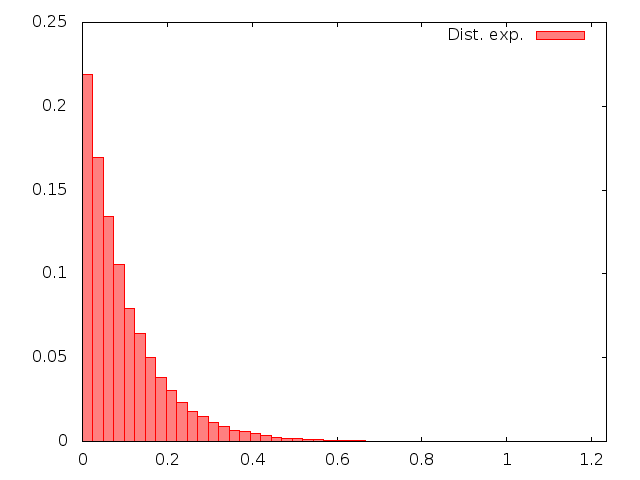
\includegraphics[width=0.5\textwidth]{DistributionExp.png}
\caption{Une loi exponentielle\label{figure:distexp}}
\end{center}
\end{figure}

%.......................................................................
%
%.......................................................................
\subsubsection{Distribution de Pareto}

   On spécifie une loi de Pareto de paramètres $\alpha$ et $x_{min}$
grâce à la  fonction suivante 

\index{randomGenerator\_setDistributionPareto}
\begin{verbatim}
void randomGenerator_setDistributionPareto(struct randomGenerator_t * rg,
                                           double alpha, double xmin);
\end{verbatim}

   La figure \ref{figure:distpa} donne un exemple de résultat obtenu
avec une distribution de Pareto de paramètres $\alpha = 40.0$ et
$x_{min} = 1.0$

\begin{figure}[h]
\begin{center}
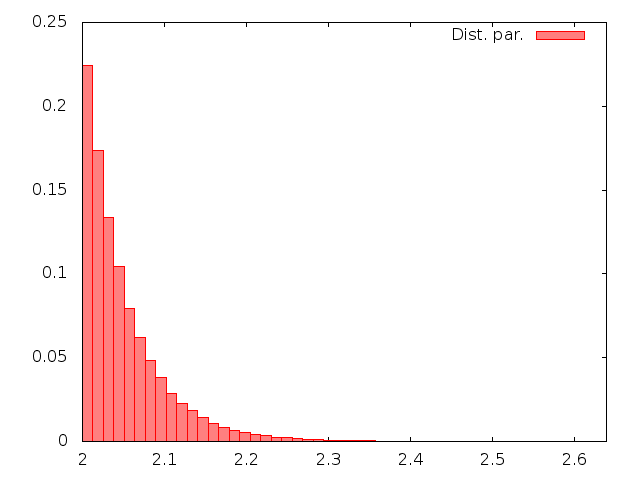
\includegraphics[width=0.5\textwidth]{DistributionPar.png}
\caption{Une loi de Pareto\label{figure:distpar}}
\end{center}
\end{figure}

%.......................................................................
%
%.......................................................................
\subsubsection{Distribution de Pareto tronquée}


%.......................................................................
%
%.......................................................................
\subsubsection{Distribution Log normale tronquée}


%.......................................................................
%
%.......................................................................
\subsubsection{Loi  explicite}

   Je ne sais pas trop comment l'appeler celle-là ! L'idée est qu'on
fournit explicitement toutes les probabilités. Elle est spécifiée par
la fonction suivante :

\index{randomGenerator\_setDistributionDiscrete}
\begin{verbatim}
void randomGenerator_setDistributionDiscrete(struct randomGenerator_t * rg,
					     int nb,
                                             double * proba);
\end{verbatim}

   Attention, elle ne s'applique de toute évidence qu'à des données
discrètes !

   Les probabilités sont copiées par la fonctions donc le pointeur
{\tt proba} peut être libéré ensuite.

%------------------------------------------------------------------------
%
%------------------------------------------------------------------------
\subsection{Choix de la source}

%------------------------------------------------------------------------
%
%------------------------------------------------------------------------
\subsection{Génération d'une valeur}

\index{randomGenerator\_getNextUInt}
\index{randomGenerator\_getNextDouble}

   Une nouvelle valeur est obtenue à chaque appel d'une des fonctions
suivantes (à choisir en fonction du type attendu)

\begin{verbatim}
unsigned int randomGenerator_getNextUInt(struct randomGenerator_t * rg);
double randomGenerator_getNextDouble(struct randomGenerator_t * rg);
\end{verbatim}

%------------------------------------------------------------------------
%
%------------------------------------------------------------------------
\subsection{Les sondes}

   Il n'existe pour le moment qu'un seul point d'ancrage pour les
sondes : sur les valeurs générées par un générateur aléatoire. Ces
valeurs sont donc converties en {\tt double} avant d'être
échantillonnées.

   La fonction permettant de placer une telle sonde est la suivante 

\index{randomGenerator\_addValueProbe}
\begin{verbatim}
void randomGenerator_addValueProbe(struct randomGenerator_t * rg,
				   struct probe_t * p);
\end{verbatim}

   Je pense que cela se passe de commentaire, \ldots

%------------------------------------------------------------------------
%
%------------------------------------------------------------------------
\subsection{Le coin du programmeur}

   Tout ce qui précède est suffisant pour l'utilisateur. En revanche,
comme d'habitude, pour le programmeur, les choses se compliquent un
peu.

   Comme souligné précédemment, les générateurs aléatoires sont
composés de trois parties. Voyons ici comment elles sont implantées et
peuvent être étendues.

%.......................................................................
%
%.......................................................................
\subsubsection{Les sources d'aléa}

%.......................................................................
%
%.......................................................................
\subsubsection{Les distributions}

%.......................................................................
%
%.......................................................................
\subsubsection{Définition par la fonction inverse de la {\sc cdf}}

   Certaines distributions peuvent être simulées en se fondant sur la
fonction réciproque de la fonction  de répartition. {\sc Ndes} propose
des outils pour cela.

%.......................................................................
%
%.......................................................................
\subsubsection{Les types}
